%!TEX root = ../../super_main.tex

\section{Sensor Providers}
\label{sec:sensor_providers}

We have implemented a threaded abstraction over the different data sources that the system should utilize in order to gather context for the labels that will eventually be combined to form the output training data for the system. The abstraction is threaded because we want the Android application to be able to gather information from multiple sources concurrently. This is done in order to make sure that the gathered data is obtained temporally close to when the label for the data was obtained. 

\subsection{Data Quantity Estimation}
\label{sub:data_quantity_estimation}

%This gave us a dataset with a size of 142908 bytes. This experiment would then yield a data set of approximately 205 MB if it was run for a day. Running the same experiment for 30 days with 100 different devices would then approximately yield a data set of 617 GB assuming similar mobile devices with similar sensors. This quick napkin math was only for one sensor with 100 people and this could quickly escalate if more sensor or more people are added. 
As described in \secref{sec:deriving_the_context_from_sensors}, some sensor measurements are continuous. We have experimented with different continuous sensors on a Nexus 5 smartphone and logged all values captured from the sensor for 1, 5, 20 minutes. The results of these tests can be seen in \tabref{tab:sensor_experiment}. Note that the orientation sensor is a virtual sensor, which uses data collected from both the gyroscope and magnetometer, hence the correlation between the data sizes ($143 \text{KB} + 35 \text{KB} \approx 177 \text{KB}$ for 1 minute). These tests were only performed for four different sensors, but customers might need data from several different sensors, thus further increasing the amount of data collected. One should also consider that this data is only collected for a single phone / person. Collecting the data from several phones / people would further escalate the total collected data size. These quantities of data might present a problem even on modern mobile platforms due to paid limited data plans and battery consumption. There might be different data needs, some customers might require very detailed data from many sensors from a few devices and others might require more sparse data from a few sensors from a lot of different devices. 

\begin{table}[!htbp]
\centering
\begin{tabular}{l|c|c|c|c}
\textbf{Sensor}     & \textbf{Accellerometer} & \textbf{Gyroscope} & \textbf{Magnetometer} & \textbf{Orientation} \\ \hline
\textbf{1 minute}   & 142 KB                  & 143 KB             & 35 KB                 & 177 KB               \\ \hline
\textbf{5 minutes}  & 714 KB                  & 714 KB             & 178 KB                & 892 KB               \\ \hline
\textbf{20 minutes} & 2859 KB                 & 2859 KB            & 715 KB                & 3573 KB                
\end{tabular}
\caption{Data size of sensor data collection after a set amount of time.}
\label{tab:sensor_experiment}
\end{table}
\FloatBarrier

% Træls for bruge
% Træls for folk der kan bruge data

\subsection{Temporality}

% Det bliver hurtigt til meget data når man arbejder med continious data
% Vi bruger sample frequency til at lave mellemrum mellem samples i tid fordi det ikke er så brugbart at have 8gb data for et minuts målinger
% Vi vil gerne have flere measurements per sample så vi kan undgå upræcise målinger

We have come up with a solution to the concerns described in \secref{sub:data_quantity_estimation}. We have decided to facilitate periodic data collection instead of continuous readings of data in order to facilitate different data needs. \figref{fig:sample_temporality} illustrates how samples are collected. A sample consists of multiple measurements to allow for further precision. Both sample frequency and measurement frequency are configurable.

\todo[inline]{Vi har reelt 3 forskellige tider: Hvor længe skal et sample vare, hvor ofte skal vi tage et sample, hvor længe skal der gå imellem measurements i et sample? På grund af at sensore i Android giver svar når de har lyst, er det ikke sikkert at der kommer den samme mængde measurements i hver sample. Vi skal overveje om det giver mening, eller om det er vigtigere for kunden at hvert sample med garenti indeholder x measures. Problemet med dette er så at vi ikke kan sætte nogen garenti for hvornår disse measures reelt kommer.} 

\begin{figure}[!htbp]
    \centering
    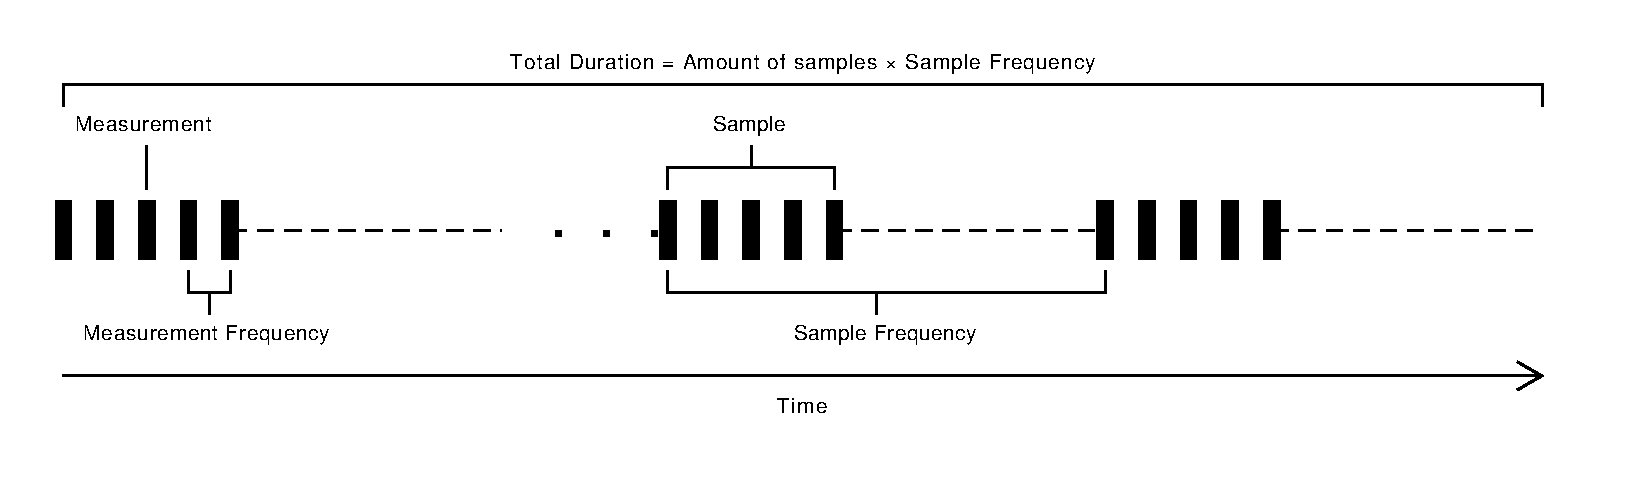
\includegraphics[width=\textwidth]{unsorted/sample_temporality}
    \caption{Overview of sample and measurement temporality.}
    \label{fig:sample_temporality}
\end{figure}
\FloatBarrier

\subsection{Implementation}

The solution was to abstract data collection away in subclasses of a class called.. \todo{Write more}

\todo[inline]{Man giver en Callable til en threadpool som så retunerer en Future. Den future indeholder så data når callablen er færdig med at gøre det den skal. Man kan kalde .get() på den future for at få dataen. Hvis dataen endnu ikke er klar venter man til den er klar. Man kan også sætte en timeout på .get() så den ikke venter mere end x sekunder (null resultat). Overvej hvornår vi skal beskrive dette i rapporten. Det ændre sig måske hvis vi finder nogle problemer med denne løsning}

% \lstinputlisting[
%    style = java,
%    caption = {Property similarity on a component.},
%    label = {lst:attribute_difference},
%]{content/implementation/annotation/attribute_difference.java}